% 第5章 低速飛行特性
%!TEX root = main.tex

%%%%%%%%%%%%%%%%%%%%%%
\chapter{低速飛行特性}
\label{flight_char}
%%%%%%%%%%%%%%%%%%%%%%

本章では,実験で得られたデータから,これまでに述べた力学モデルを用いてパラメータ同定を行ない,低速飛行時の飛行特性について検証する.まず機体が持つ固有振動をとらえるために,線形モデルによる固有値解析を行なう.次に,同定を行なった結果から,提案モデルの妥当性を検討する.最後に,同定結果をCFD解析の結果と比較し,考察を行なう.

%%%%%%%%%%%%%%%%%%%%%%%%%%%%%%%%%%%%
\section{線形モデルによる固有値解析}
\label{sec:analyze}
%%%%%%%%%%%%%%%%%%%%%%%%%%%%%%%%%%%%

本節では,線形化された機体の飛行モデルを用いて,固有値解析を行なう.まず,式(\ref{eq:lin_model})より,$\Delta$を省略して微分方程式をまとめると
\begin{equation}
  \dfrac{d}{dt}
  \underbrace{
  \left[
  \begin{array}{cccc}
    u \\
    \alpha \\
    q \\
    \theta \\
  \end{array}
  \right]}_{\underline{x}} =
  \underbrace{
  \left[
  \begin{array}{cccc}
    X_u & X_\alpha & X_q & X_\theta \\
    \overline{Z_u} & \overline{Z_\alpha} & \overline{Z_q} & \overline{Z_\theta} \\
    \overline{M_u} & \overline{M_\alpha} & \overline{M_q} & \overline{M_\theta} \\
    0 & 0 & 1 & 0
  \end{array}
  \right]}_{A}
  \underbrace{
  \left[
  \begin{array}{cccc}
    u \\
    \alpha \\
    q \\
    \theta \\
  \end{array}
  \right]}_{\underline{x}} +
  \underbrace{
  \left[
  \begin{array}{cccc}
    X_{\delta_e} & X_{T_m} & 0 & 0 \\
    \overline{Z_{\delta_e}} & \overline{Z_{T_m}} & \overline{Z_{T_r}} & \overline{Z_{T_f}} \\
    \overline{M_{\delta_e}} & \overline{M_{T_m}} & \overline{M_{T_r}} & \overline{M_{T_f}} \\
    0 & 0 & 0 & 0
  \end{array}
  \right]}_{B}
  \underbrace{
  \left[
  \begin{array}{cccc}
    \delta_e \\
    T_m \\
    T_r \\
    T_f \\
  \end{array}
  \right]}_{\underline{u}}
  \label{eq:system_eq}
\end{equation}
となる.プロセスノイズを省略すれば,この状態方程式は行列$A,B$と状態量$\underline{x}$,入力$\underline{u}$を用いることによって
\begin{equation}
  \dfrac{d\underline{x}}{dt} = A\underline{x} + B\underline{u}
\label{eq:matrix_A}
\end{equation}
と表すことができる.したがってこれを連続時間システムとすれば,一般に
\begin{equation}
  \underline{x}(t) = e^{At}\underline{x}(0) + \int_0^t e^{A(t-\tau)}B\underline{u}(\tau) d\tau
  \label{eq:system}
\end{equation}
が得られる.式(\ref{eq:system})の右辺第1項目は,斉次方程式の一般解であり,行列$A$の固有値に従う挙動を示す.右辺第2項目は特殊解であり,入力$\underline{u}$による振動数と行列$A$の固有値に従う挙動を示す.

% ここで入力$\underline{u}$が,振動や減衰を表す関数
% \begin{equation}
%   \underline{u} = \sum \underline{f} e^{\omega t}
% \end{equation}
% であるとする.ただし$\omega$は複素数($\omega \in \mathbb{C}$)である.これにより,状態量$\underline{x}$は解析的に解くことができ
% \begin{equation}
%   \underline{x} = \left(\sum_{i}C_i x_i e^{\lambda_i t}\right) +
%   \sum(\omega I - A)^{-1} \underline{f} e^{\omega t}
% \end{equation}
% となる.ここで右辺第1項は,ある係数$C_i$,行列$A$の固有値$\lambda_i$,固有ベクトル$x_i$で表された一般解で,状態に固有な振動や発散,減衰などを表している.右辺第2項は特殊解であり,入力と同じ周波数成分を持つ.つまり,外乱がない限り,状態量は周波数成分として固有振動数や入力に存在する周波数成分に相関するということである.


そこで,\ref{sec:filter}小節でも述べたように,固有振動数を計算することで機体の運動が持つおおよその周波数帯をつかみ,データのフィルタリングに利用する.実際に式(\ref{eq:matrix_A})の行列$A$について,固有値を計算して絶対値をプロットしたものがFig. \ref{fig:eigen},\ref{fig:eigen_nondalpha}である.Fig. \ref{fig:eigen}は,提案モデルをそのまま用いて同定した結果から固有値を計算したものである.一方Fig. \ref{fig:eigen_nondalpha}は,提案モデル内の空力係数から$\dot{\alpha}$を含む項を除いて同定した結果から固有値を計算したものである.ただし,式(\ref{eq:system_eq})で示した行列$A$の上線を付した要素は,上線を除いた要素に置き換えられる.行列$A$が4次の正方行列であるため,各データ点ごとに最大4つの固有値を持ち,それぞれ色分けされている.グラフ内の縦破線は,複数の実験データそれぞれの境界を示す.

Fig. \ref{fig:eigen}では,固有値の絶対値が50よりも大きいものが存在するが,開発機体は$50\mbox{[Hz]}$の周波数をもつ制御系で安定化できているため,機体の持つ固有振動数としては適切でないと考えられる.そこで,Table \ref{tb:si_result}で示した同定結果を見ると,$\dot{\alpha}$と$q$の安定微係数の値は符号の異なる絶対値の近い値であることがわかる.それぞれ他の係数と比較しても妥当な値とは言えず,$\dot{\alpha}$および$q$の関係が独立でない可能性が考えられる.これに関しては,今後の課題として結論で詳細を述べる.

以上を踏まえ,$\dot{\alpha}$を含む項を除いて同定した結果をTable \ref{tb:si_result_nondalpha}に示し,これを用いて固有値を計算した結果をFig. \ref{fig:eigen_nondalpha}に示している.

\begin{figure}[H]
	\centering
	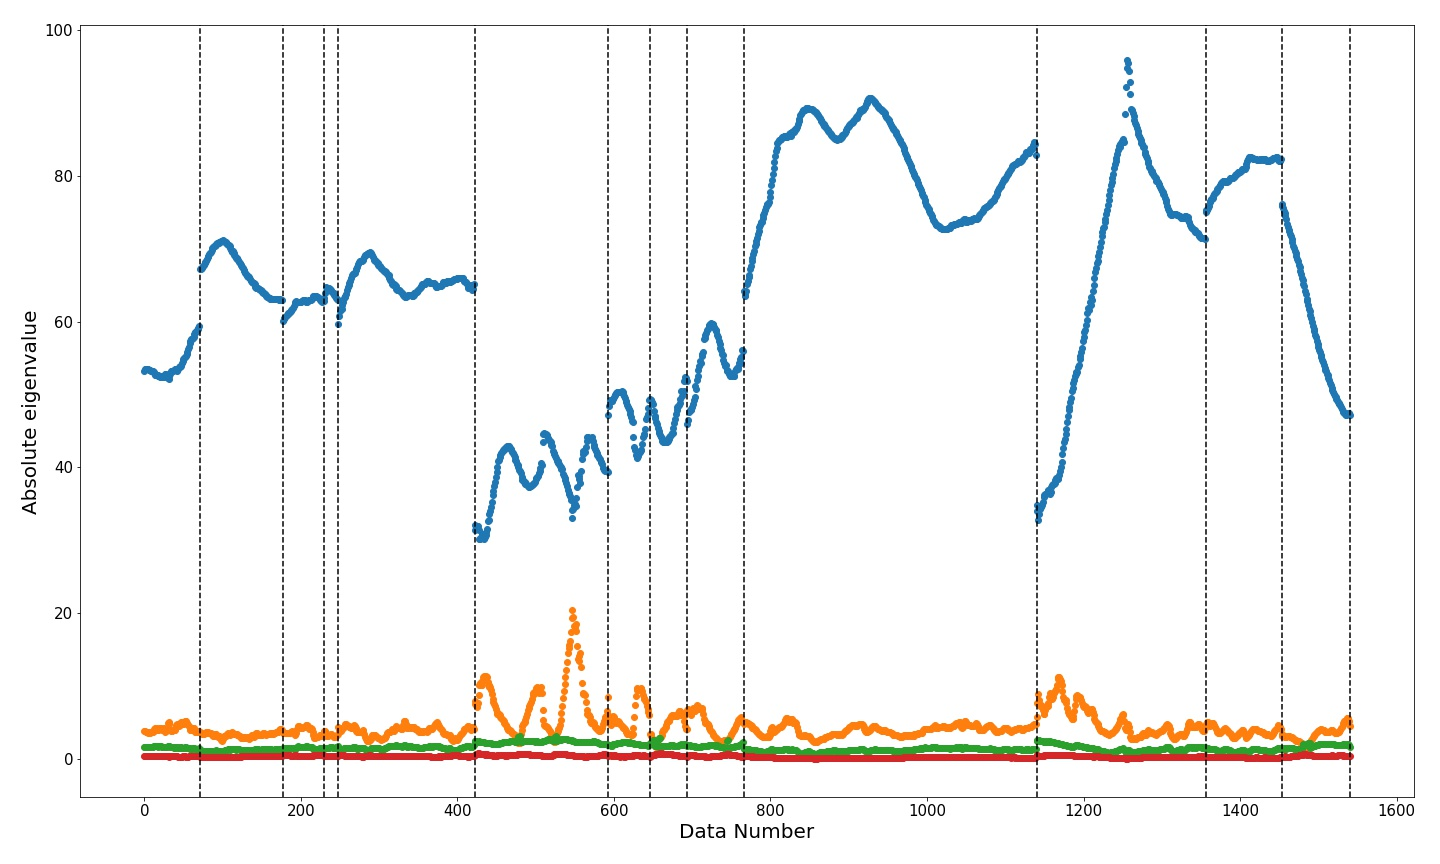
\includegraphics[clip,width=9.0cm,bb=0 0 1440 864]{./z_figure_files/chapter5/eigen_bad.jpeg}
	\caption{Absolute value of eigenvalue of matrix A}
	\label{fig:eigen}
\end{figure}

\begin{figure}[H]
	\centering
	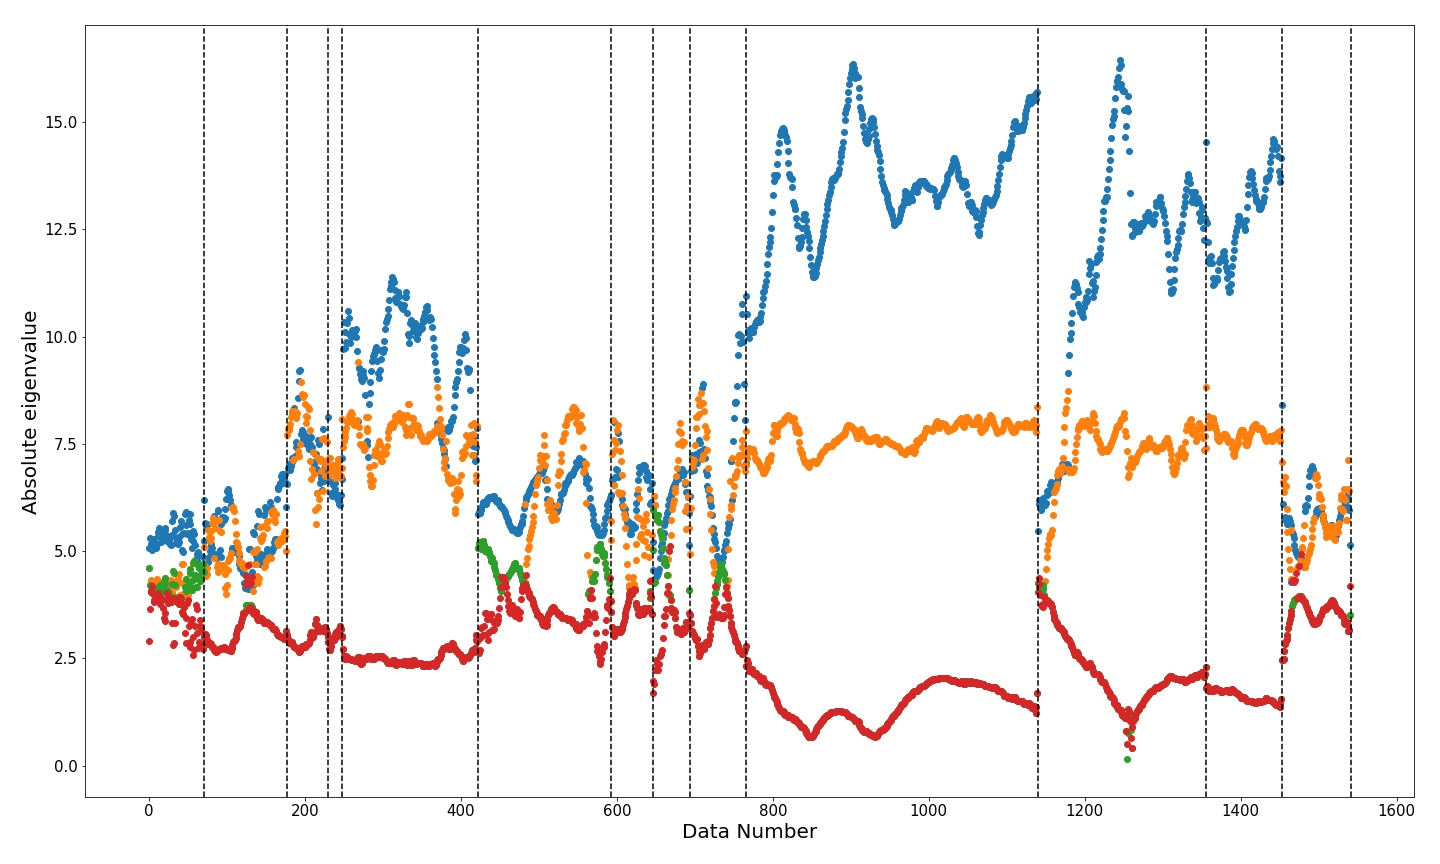
\includegraphics[clip,width=9.0cm,bb=0 0 1440 864]{./z_figure_files/chapter5/eigen_good.jpeg}
	\caption{Absolute value of eigenvalue of matrix A without $\dot{\alpha}$}
	\label{fig:eigen_nondalpha}
\end{figure}

\begin{table} [htbp]
  \begin{center}
    \caption{Identified parameters without $\dot{\alpha}$}
    \label{tb:si_result_nondalpha}
    \begin{tabular}{|c||r|cc||r|} \hline
      $C_{L_0}$ & 0.5153 & & $C_{m_0}$ & 1.318 \\ \hline
      $C_{L_\alpha}$ & 1.484 & & $C_{m_\alpha}$ & -0.1126 \\ \hline
      $C_{L_q}$ & 2.724 & & $C_{m_q}$ & 1.307\\ \hline
      $C_{L_{\delta_e}}$ & -1.330 & & $C_{m_{\delta_e}}$ & 0.3632 \\ \hline
      $C_{L_k}$ & -5.224 & & $C_{m_k}$ & -7.750 \\ \hline
      $C_{D_0}$ & 0.9647 &&&\\ \hline
      $\kappa$ & 0.6798 &&&\\ \hline
      $C_{D_k}$ & 0.7904 &&&\\ \hline
    \end{tabular}
  \end{center}
\end{table}

%%%%%%%%%%%%%%%%%%%%%%%%%%%%
\section{空気力モデルの検証}
\label{sec:airf_model_ver}
%%%%%%%%%%%%%%%%%%%%%%%%%%%%

本節では,パラメータ同定の結果から,提案モデルが妥当であるかを考える.Fig. \ref{fig:CL_si}〜\ref{fig:Cm_si}にはそれぞれ3種類の色分けされた点がプロットされている.これらは以下に示す3通りのデータセットをプロットしている.

\begin{itemize}
  \setlength{\leftskip}{1.0cm}
  \setlength{\rightskip}{0.5cm}
  \item[Data1(青)] $L_{log},D_{log},M_{a_{log}}$を用いて,各ステップごとに算出した空力係数群\\(ログデータから得られた,真値に近いと考えられる値)
  \item[Data2(黄)] 式(\ref{eq:L_o})〜(\ref{eq:Ma_o}),すなわち$k_* V_a$の項を除いた従来モデルを用いて同定した結果から,各ステップごとに算出した空力係数群
  \item[Data3(緑)] 式(\ref{eq:L})〜(\ref{eq:Ma}),すなわち$k_* V_a$の項を含む提案モデルを用いて同定した結果から,各ステップごとに算出した空力係数群
\end{itemize}

ただし,式(\ref{eq:CL}),~(\ref{eq:Cm})より空力係数に関係する変数は,$\alpha,\dot{\alpha},q,\delta_e,V_a$の計5個あるが,その中から$V_a$を横軸にとった場合を図示している.

$C_L$は各データセット間でそれほど大きな差は見られないが,$C_D,C_m$においては,Data1が真値に近い値であると考えれば,Data2よりもData3のほうが,よりData1に沿うように点在していることが分かる.

さらに詳細にモデルを評価するための精度評価指標として,平均平方二乗誤差(Root Mean Square Error,RMSE)を用いる.$k$番目のステップにおけるData1の値を実測値として$C_{obs,k}$,比較対象とするデータセットの値を予測値として$C_{pred,k}$とすると
\begin{equation}
  \mbox{RMSE} = \sqrt{\dfrac{1}{N}\sum_{k}(C_{obs,k}-C_{pred,k})^{2}} \quad (N\mbox{:サンプルデータ数})
  \label{eq:rmse}
\end{equation}
となる\cite{}.式(\ref{eq:rmse})を用いて,各空力係数に対して計算した結果をTable \ref{tb:rmse}に示す.結果から,Data2よりもData3のほうが,誤差は小さく予測精度が高いことがわかる.

したがって,回転翼機モードの空気力モデルにおいては,$k_* V_a$の項を含めることが妥当であると考えられる.特に,$C_D$における$k_D V_a$の効果が大きく,この結果は従来研究\cite{}の結果とも整合する.

\begin{table} [htbp]
  \begin{center}
    \caption{Comparing RMSE values}
    \label{tb:rmse}
    \begin{tabular}{|c||c|r|} \hline
      ~ & Data set & RMSE value \\ \hline \hline
      $C_L$ & Data2 & 0.4045 \\
       & Data3 & 0.3443 \\ \hline
       $C_D$ & Data2 & 0.5764 \\
        & Data3 & 0.3883 \\ \hline
        $C_m$ & Data2 & 0.8432 \\
         & Data3 & 0.7419 \\ \hline
    \end{tabular}
  \end{center}
\end{table}

\begin{figure}[htbp]
	\begin{center}
		\begin{tabular}{c}
			\begin{minipage}{0.5\hsize}
				\begin{center}
					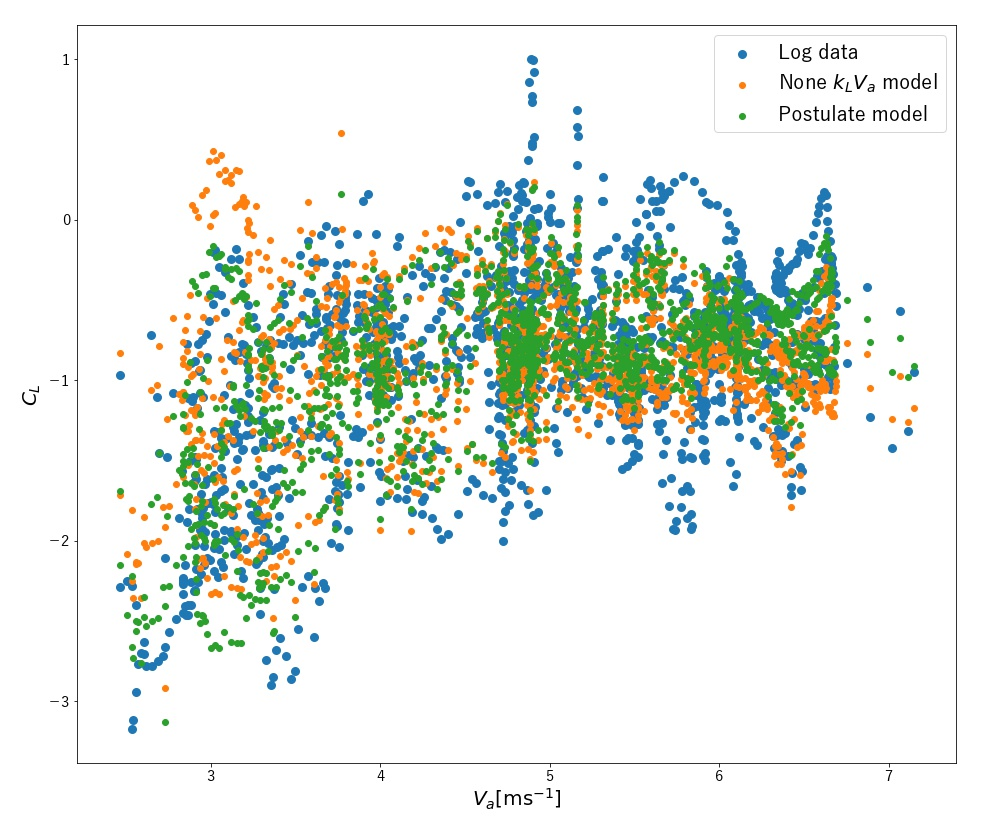
\includegraphics[clip,width=7.5cm,bb=0 0 864 654]{./z_figure_files/chapter5/2_CL.jpeg}
					\caption{$C_L$ plots}
					\label{fig:CL_si}
				\end{center}
			\end{minipage}
			\begin{minipage}{0.5\hsize}
				\begin{center}
					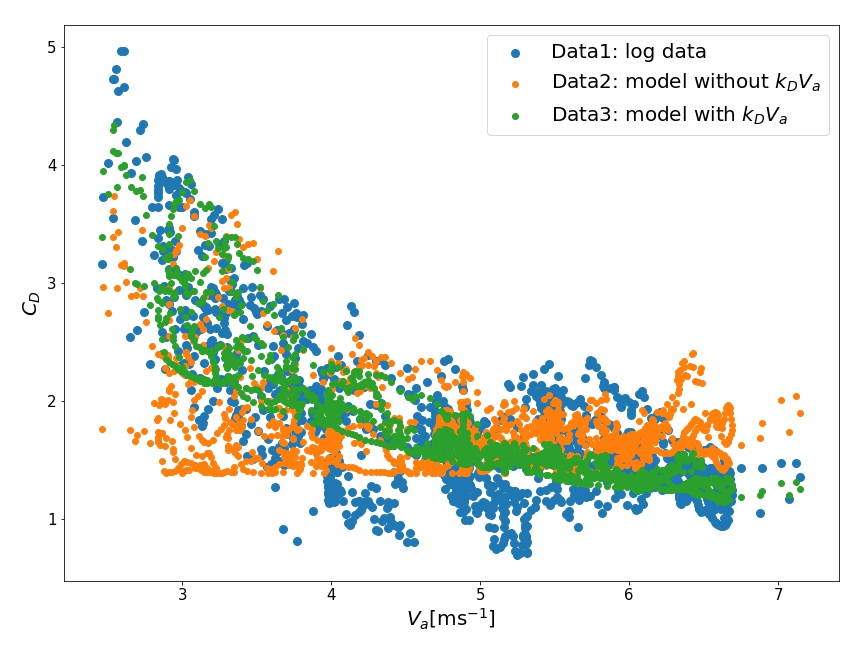
\includegraphics[clip,width=7.5cm,bb=0 0 864 654]{./z_figure_files/chapter5/3_CD.jpeg}
					\caption{$C_D$ plots}
					\label{fig:CD_si}
				\end{center}
			\end{minipage}
		\end{tabular}
	\end{center}
\end{figure}
\begin{figure}[H]
  \begin{center}
    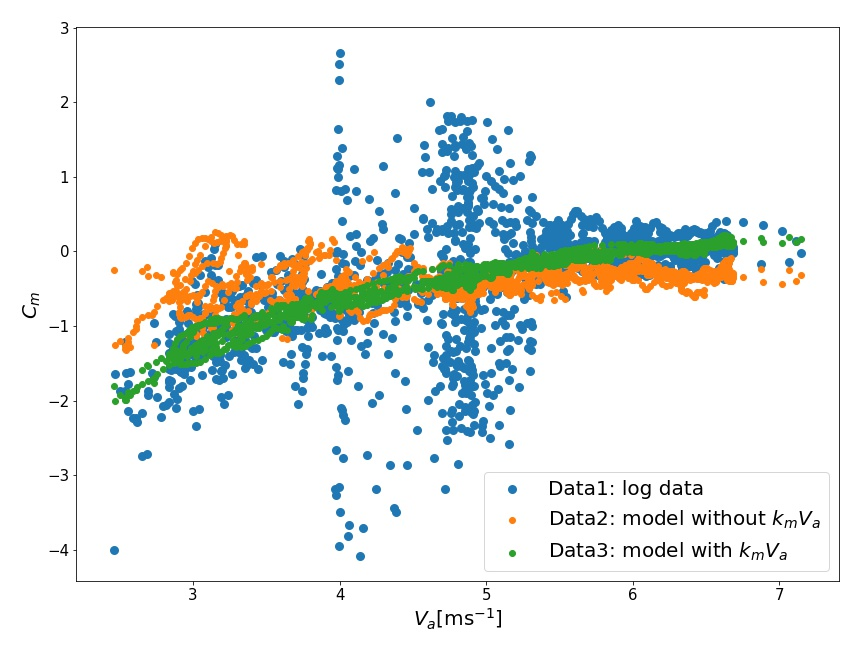
\includegraphics[clip,width=7.5cm,bb=0 0 864 654]{./z_figure_files/chapter5/4_Cm.jpeg}
    \caption{$C_m$ plots}
    \label{fig:Cm_si}
  \end{center}
\end{figure}


%%%%%%%%%%%%%%%%%%%%%%%%%%%%%%%
\section{CFDによる解析結果との比較}
\label{sec:cfd}
%%%%%%%%%%%%%%%%%%%%%%%%%%%%%%%

本節では,パラメータ同定結果の妥当性をさらに検証するために,\cite{kawano}で得られた対気速度$V_a=5\mathrm{[m s^{-1}]}$のCFD解析結果とも比較する.このため,\ref{sec:airf_model_ver}節で示したData2,Data3のデータセットから,$4.5\mathrm{[m s^{-1}]} \leq V_a \leq 5.5\mathrm{[m s^{-1}]}$であるものを選んで比較した.Fig. \ref{fig:cfd_L}〜\ref{fig:cfd_Ma}に,迎角$\alpha$を横軸にとり,揚力・抗力・ピッチモーメントそれぞれの空力係数をプロットしたものを示す.青の点($C_{*_{log}}$)がログデータから算出された値,赤の点($C_{*_{CFD}}$)がCFD解析による値,黄色の点($C_{*_{SI}}$)が同定結果をもとに,CFDに合わせて,$\alpha=-20\mathrm{[deg]},-10\mathrm{[deg]},0\mathrm{[deg]}$の3点において再現された値である.ただし,$C_{*_{CFD}}$と$C_{*_{SI}}$については$\alpha$との関係性を見るために,各点と同じ色で回帰直線を引いてある.

$C_L$について,CFDの解析結果は$\alpha$が大きいほど数値も大きくなることが見て取れる.しかし,ログデータや,特に同定結果を見ると,$\alpha$が$-5\mathrm{[deg]}$付近を境に$\alpha$の上昇に伴って数値が小さくなっていくように見える.

CFD解析では,ロータ部に加わる力と胴体および主翼等に加わる力を個別に算出している.一方で,本研究のパラメータ同定においては,機体全体に加わる力からロータで発生すると想定される力を引くことで,胴体および主翼等に加わる力を算出している.ロータで発生すると想定した力は,静止推力をもとにしており,実際の運動時の推力とずれがあると考えられる.実験時にロータで発生する推力やモーメントを正しく測定することは極めて困難であるが,運動時には静止推力に比べて実際の推力が下がっている可能性がある.この場合,実験での$C_L$の値は,CFDでの値に比べて小さくなる.

次に$C_D$について,それぞれの値のは概ね一致している.これは抗力係数のうち,迎角によって変化するとされる有害抵抗係数による影響だと考えられる\cite{katou}.同定に用いるモデルを見直す必要があると思われる.

最後に$C_m$について,ログデータにはばらつきがあるものの,どの結果も$\alpha$の値によらずほぼ一定の値を取っている.CFDの解析結果が大きく離れているのは,上述のロータ推力の推算による誤差が大きい可能性が考えられる.ロータ推力の算出方法の改善が必要である.

\begin{figure}[H]
  \centering
  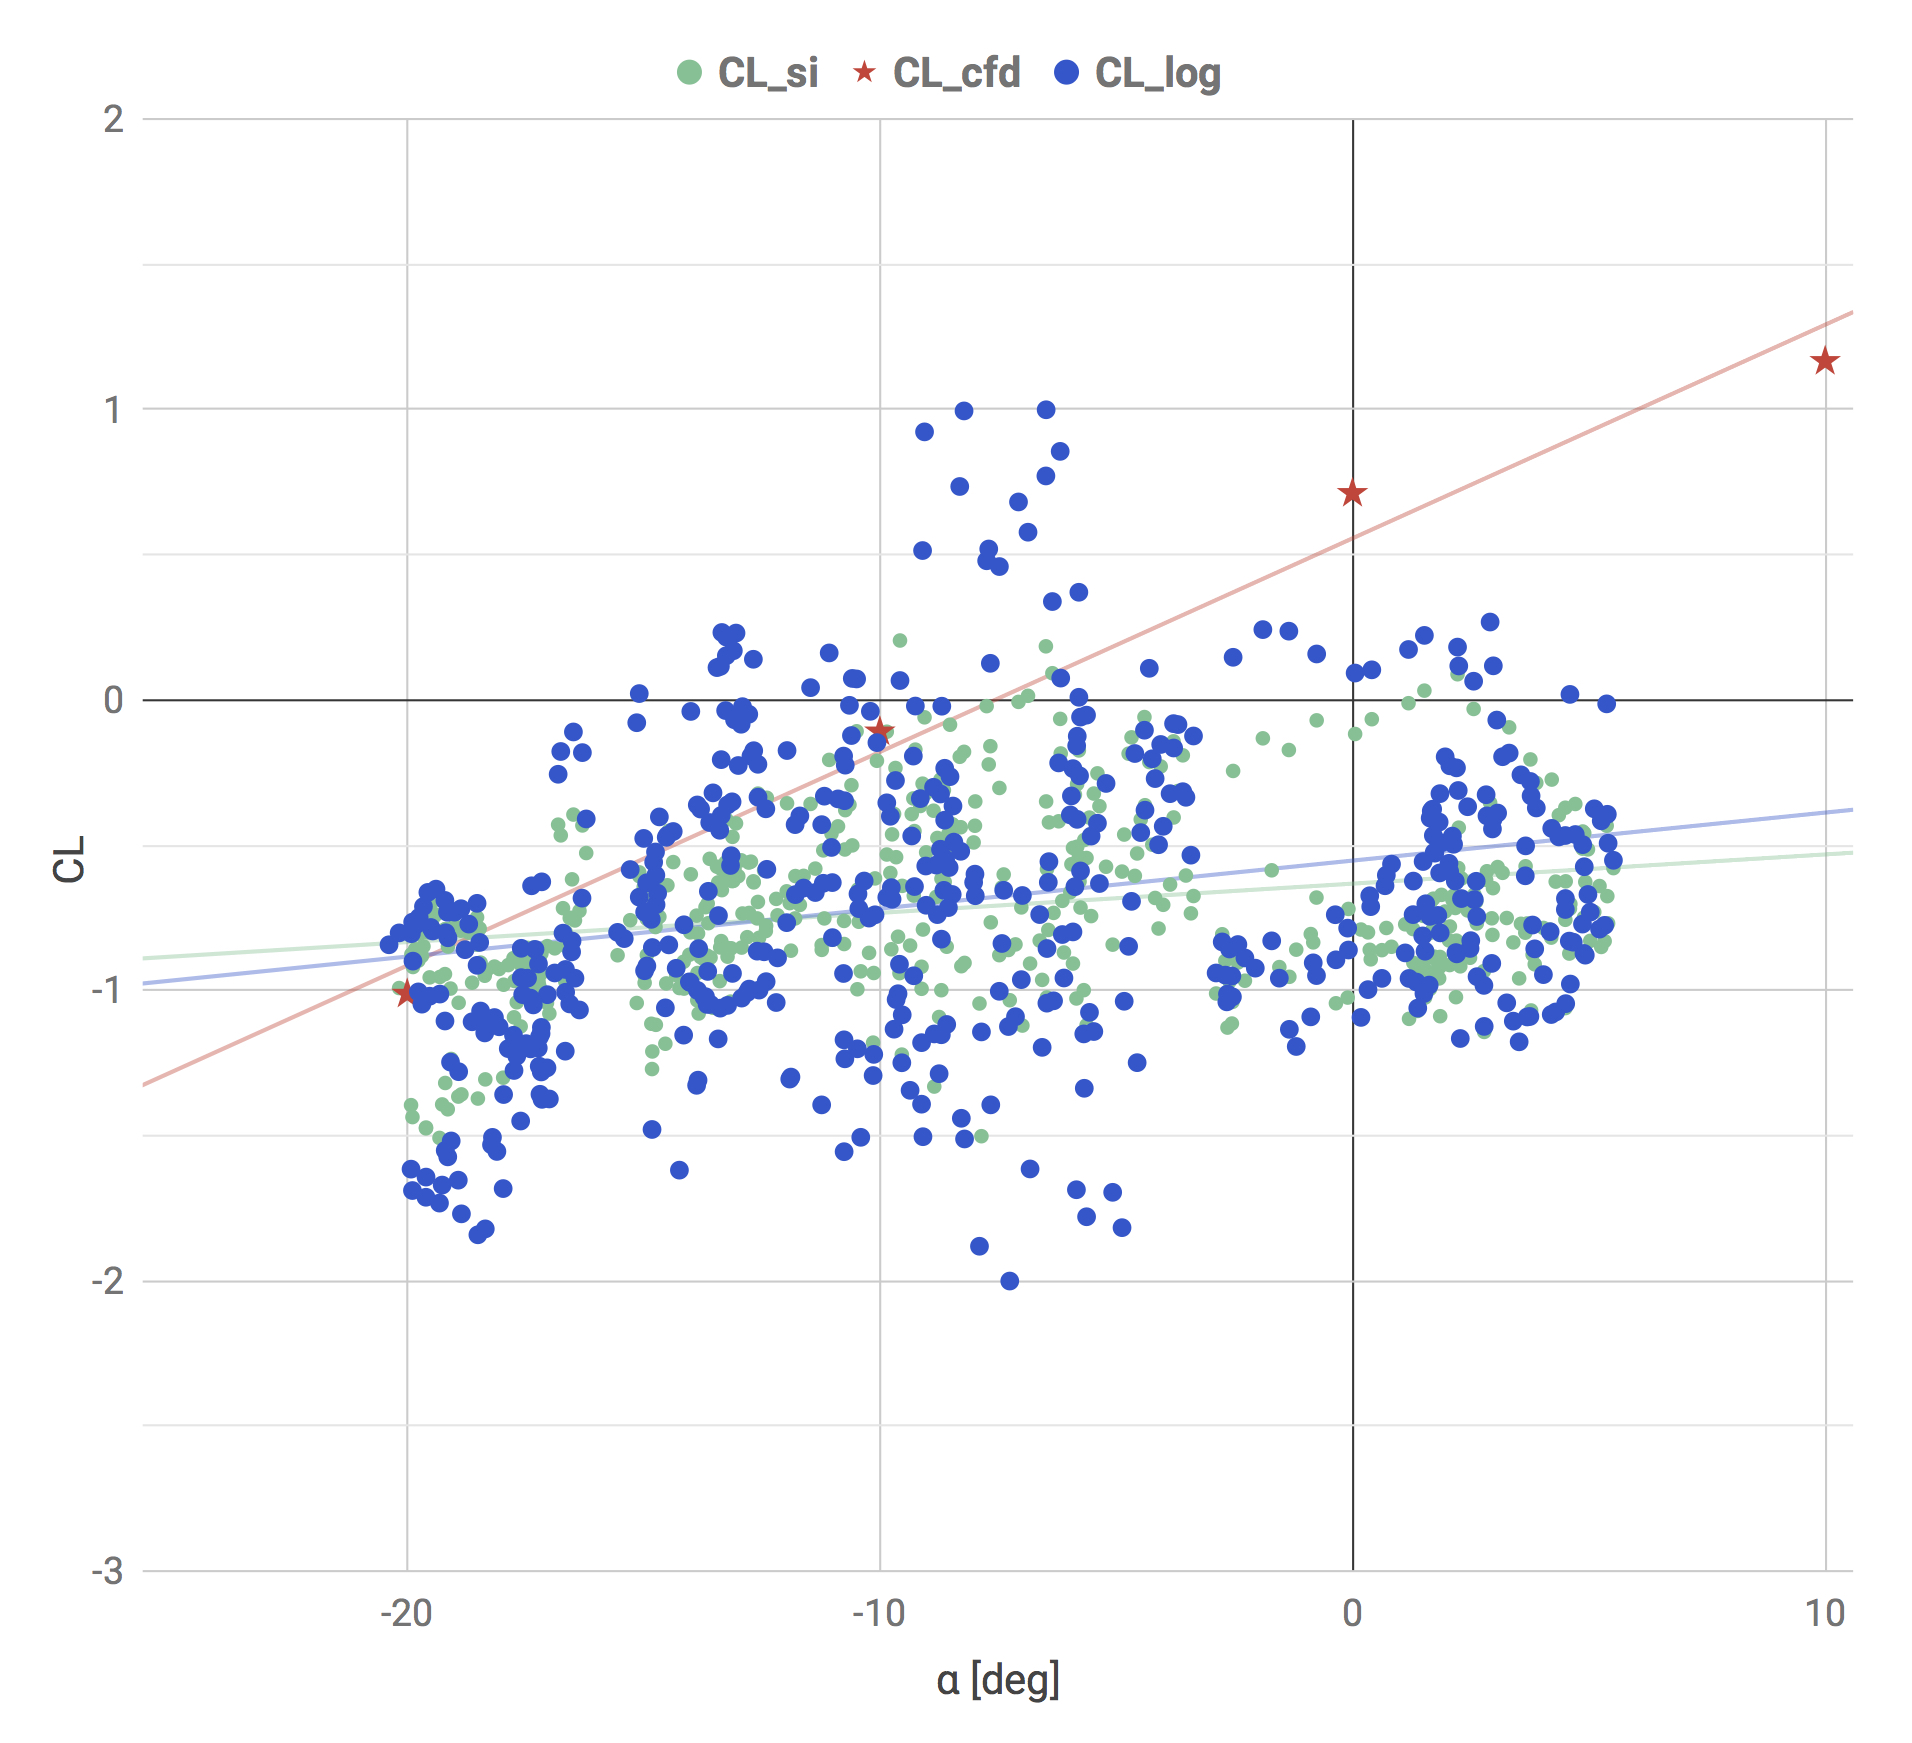
\includegraphics[clip,width=9cm,bb=0 0 1912 1743]{./z_figure_files/chapter5/cfd_L.jpeg}
  \caption{\small{Comparing $C_L$ results of CFD and identification}}
  \label{fig:cfd_L}
\end{figure}
\begin{figure}[H]
  \centering
  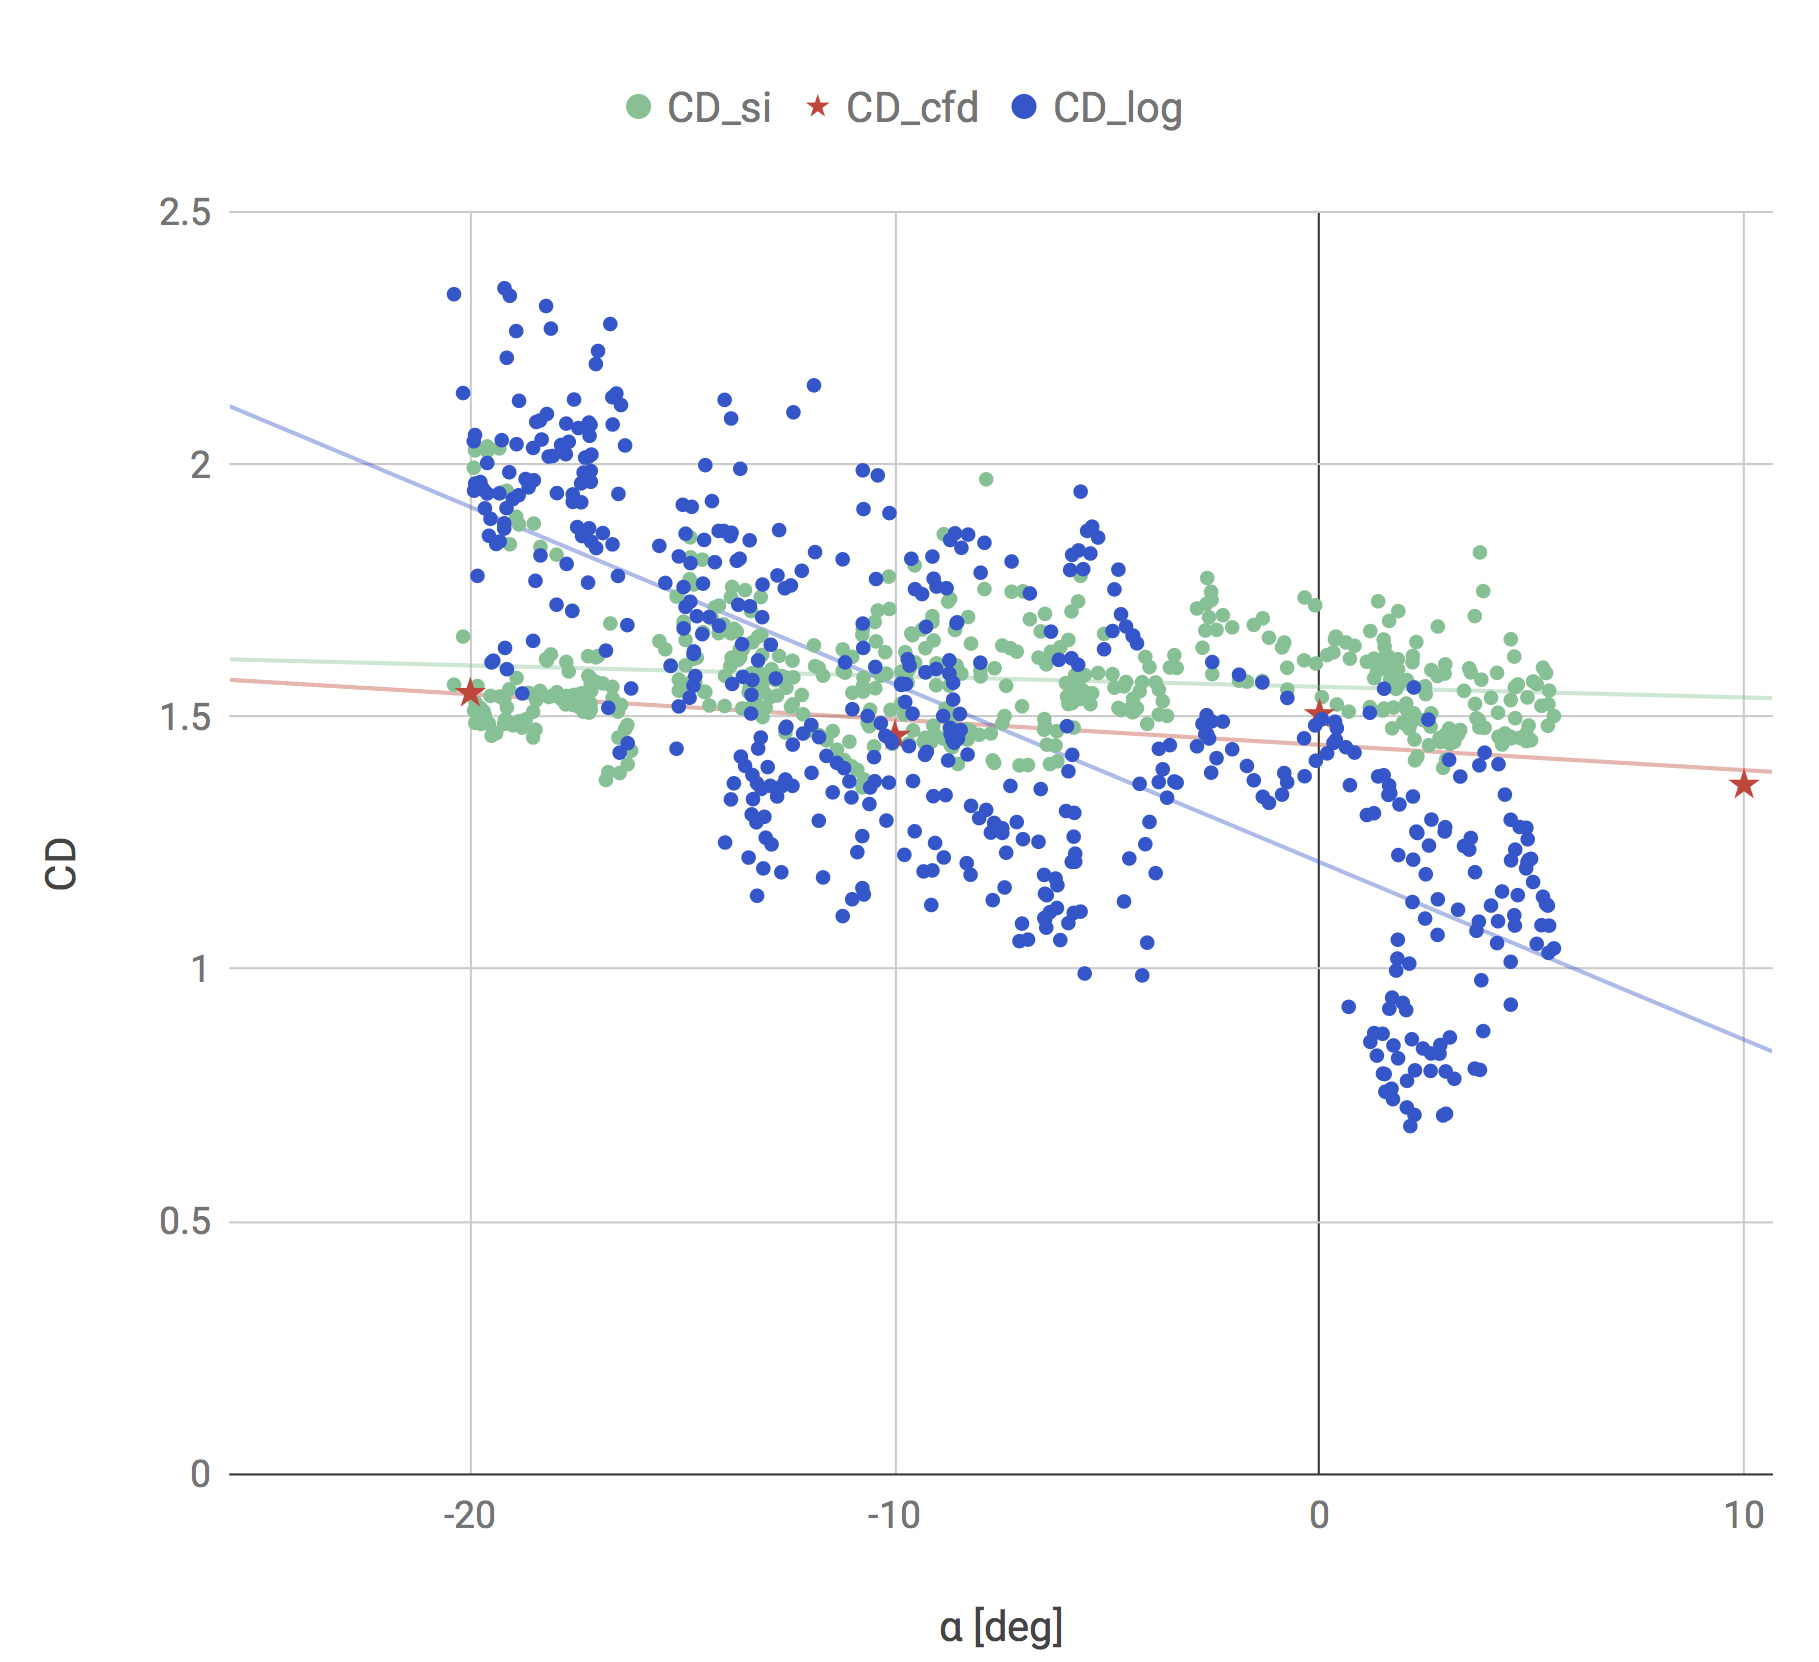
\includegraphics[clip,width=9cm,bb=0 0 1819 1662]{./z_figure_files/chapter5/cfd_D.jpeg}
  \caption{\small{Comparing $C_D$ results of CFD and identification}}
  \label{fig:cfd_D}
\end{figure}
\begin{figure}[H]
  \centering
    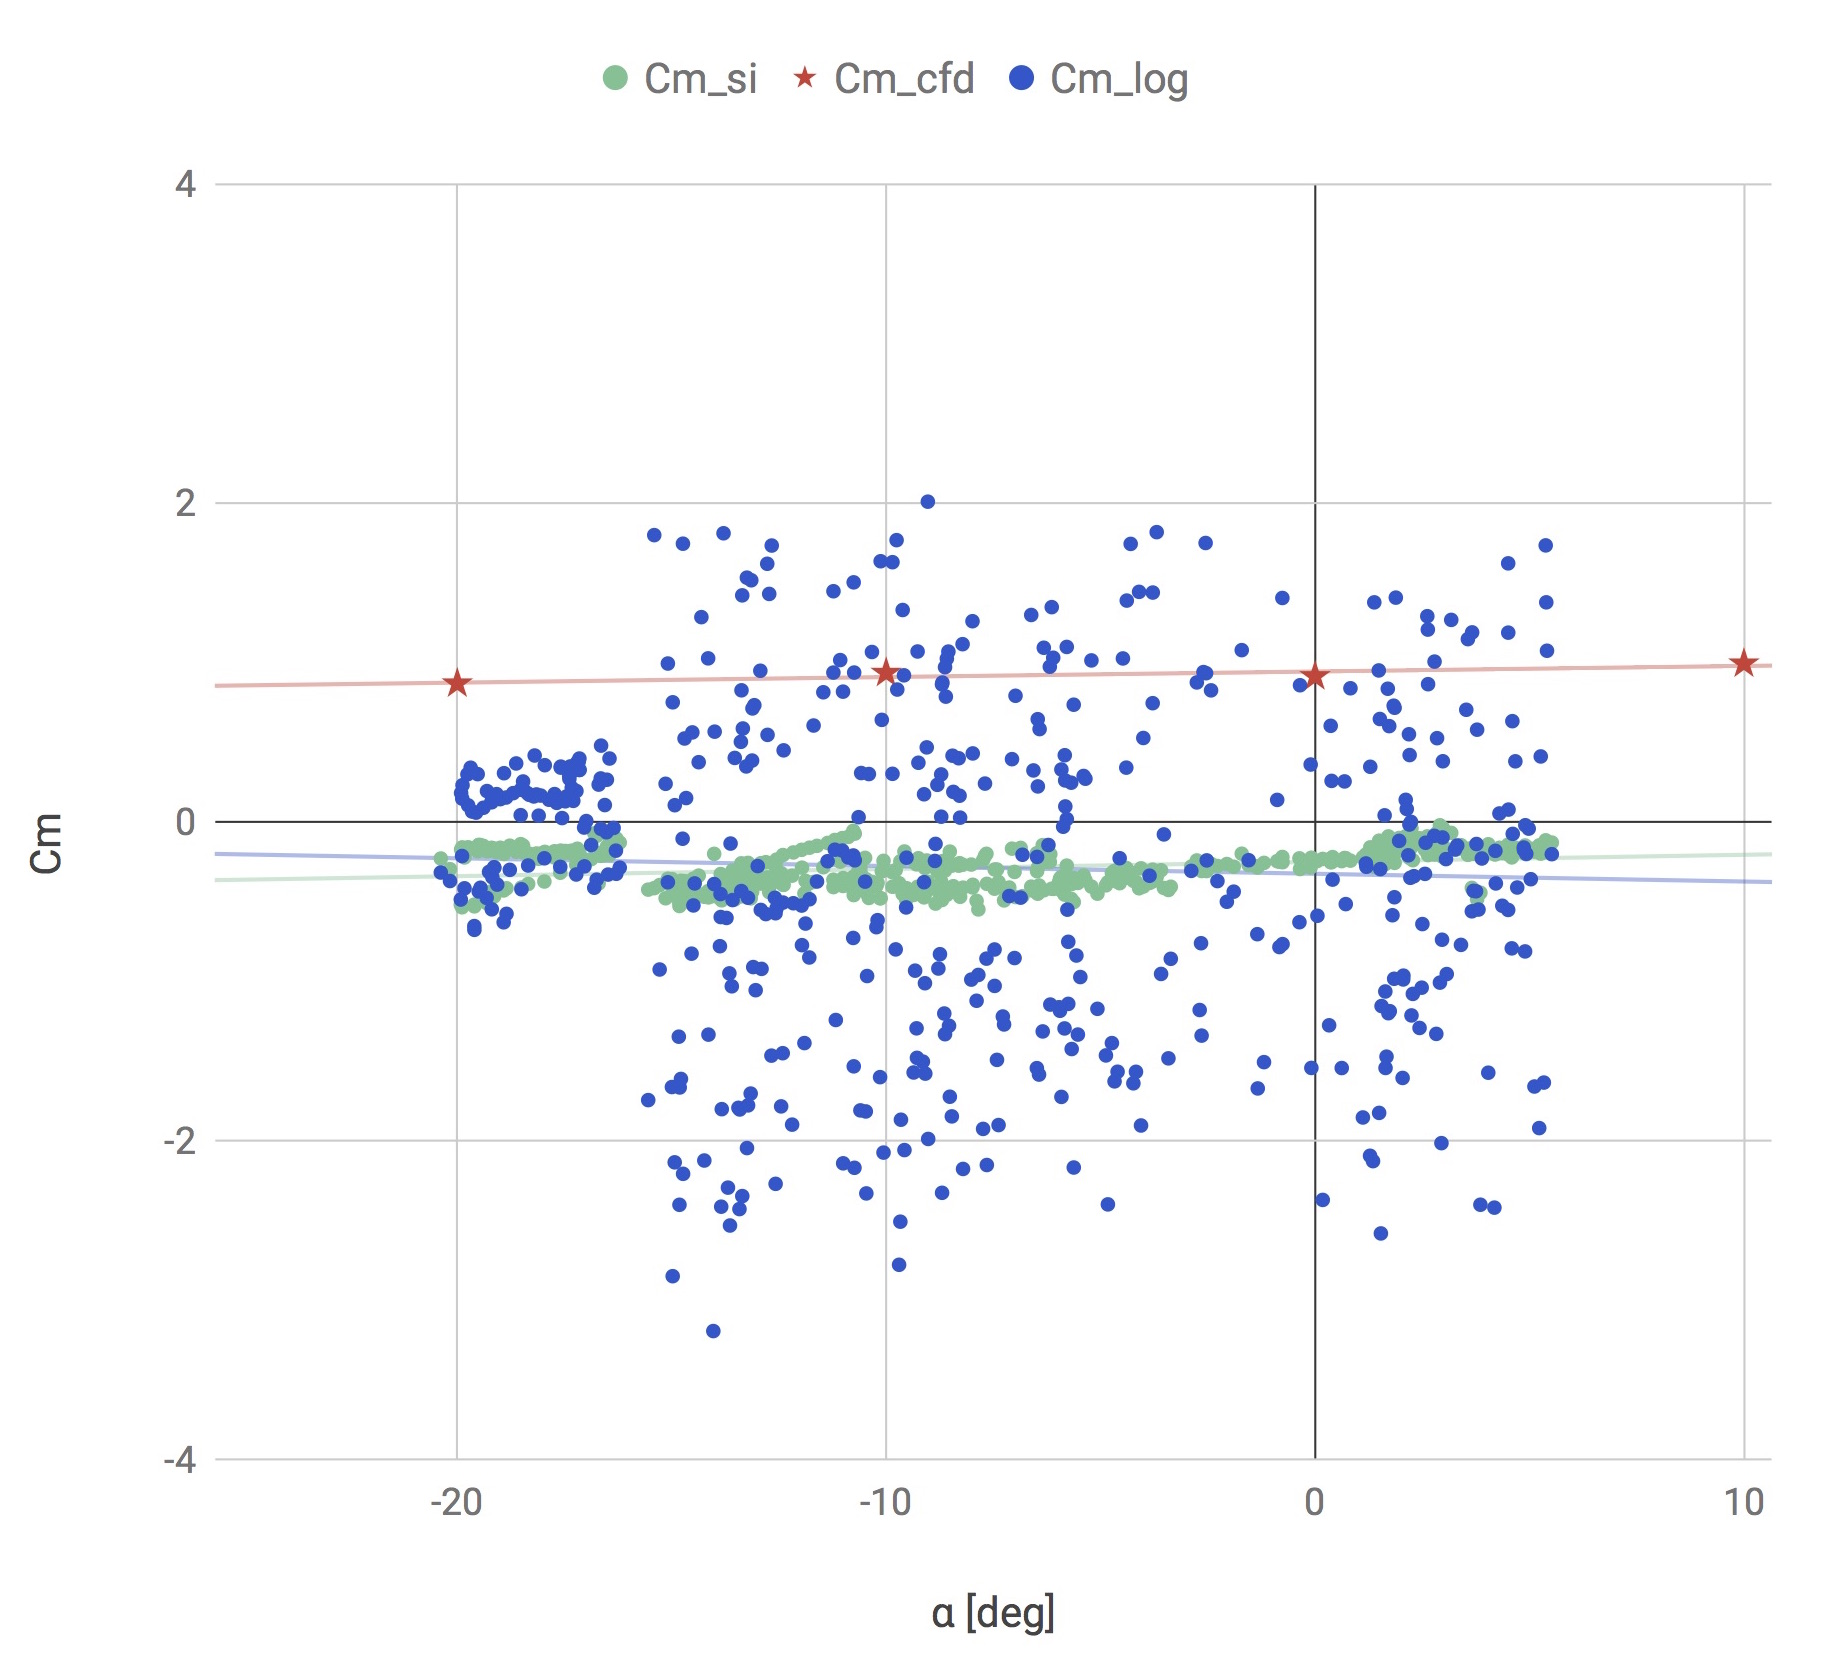
\includegraphics[clip,width=9cm,bb=0 0 1832 1662]{./z_figure_files/chapter5/cfd_m.jpeg}
    \caption{\small{Comparing $C_m$ results of CFD and identification}}
    \label{fig:cfd_Ma}
\end{figure}
